\documentclass[11pt]{lecture}

\usepackage{chronology} %% for timeline
\def\fullsize{0.55\textwidth}

\usepackage{xcolor}
\hypersetup{
    colorlinks,
    linkcolor={red!50!black},
    citecolor={blue!50!black},
    urlcolor={blue!80!black}
}

\usepackage{booktabs}
\usepackage{multirow}
% \makeatletter
% \renewcommand*{\@fnsymbol}[1]{\ensuremath{\ifcase#1\or *\or \dagger\or \ddagger\or
%     \mathsection\or \mathparagraph\or \|\or **\or \dagger\dagger
%     \or \ddagger\ddagger \else\@ctrerr\fi}}
% \makeatother
% \renewcommand{\thefootnote}{\fnsymbol{footnote}}
\begin{document}

\course{CS 6210/CS 4210 ADVANCED OPERATING SYSTEMS}
\title{Distributed Shared Memory (Part I)}%\footnotemark[1]\footnotemark[2]
\semester{Fall 2017}
\instructor{Prof. Umakishore Ramachandran}
\author{Long Gong}
\footnotetext[1]{The first several sections of this scribe are actually covered by a lecture before this one. They are included for this scribe to be self-contain.}
\footnotetext[2]{All the figures in this scribe are directly from or modified from the lecture slides provided by Prof. Umakishore Ramachandran.}
\maketitle

\section{Overview}

In this lecture we cover another way to exploit remote memories, namely 
software implementation of distributed shared memory (DSM). That is to create 
an operating system abstraction that provides an illusion of shared memory 
to the applications, even though the nodes in the local area network do not 
physically share memory. 

DSM asks the question, {\it if shared memory makes life simple for application 
development in a multiprocessor system, can we try to provide the same abstraction 
in a distributed system, and make the cluster look like a shared memory machine ?} 


\section{Motivation: Cluster as a Parallel Machine}\label{sec: motivation}

\begin{figure}[!htbp]
\centering 
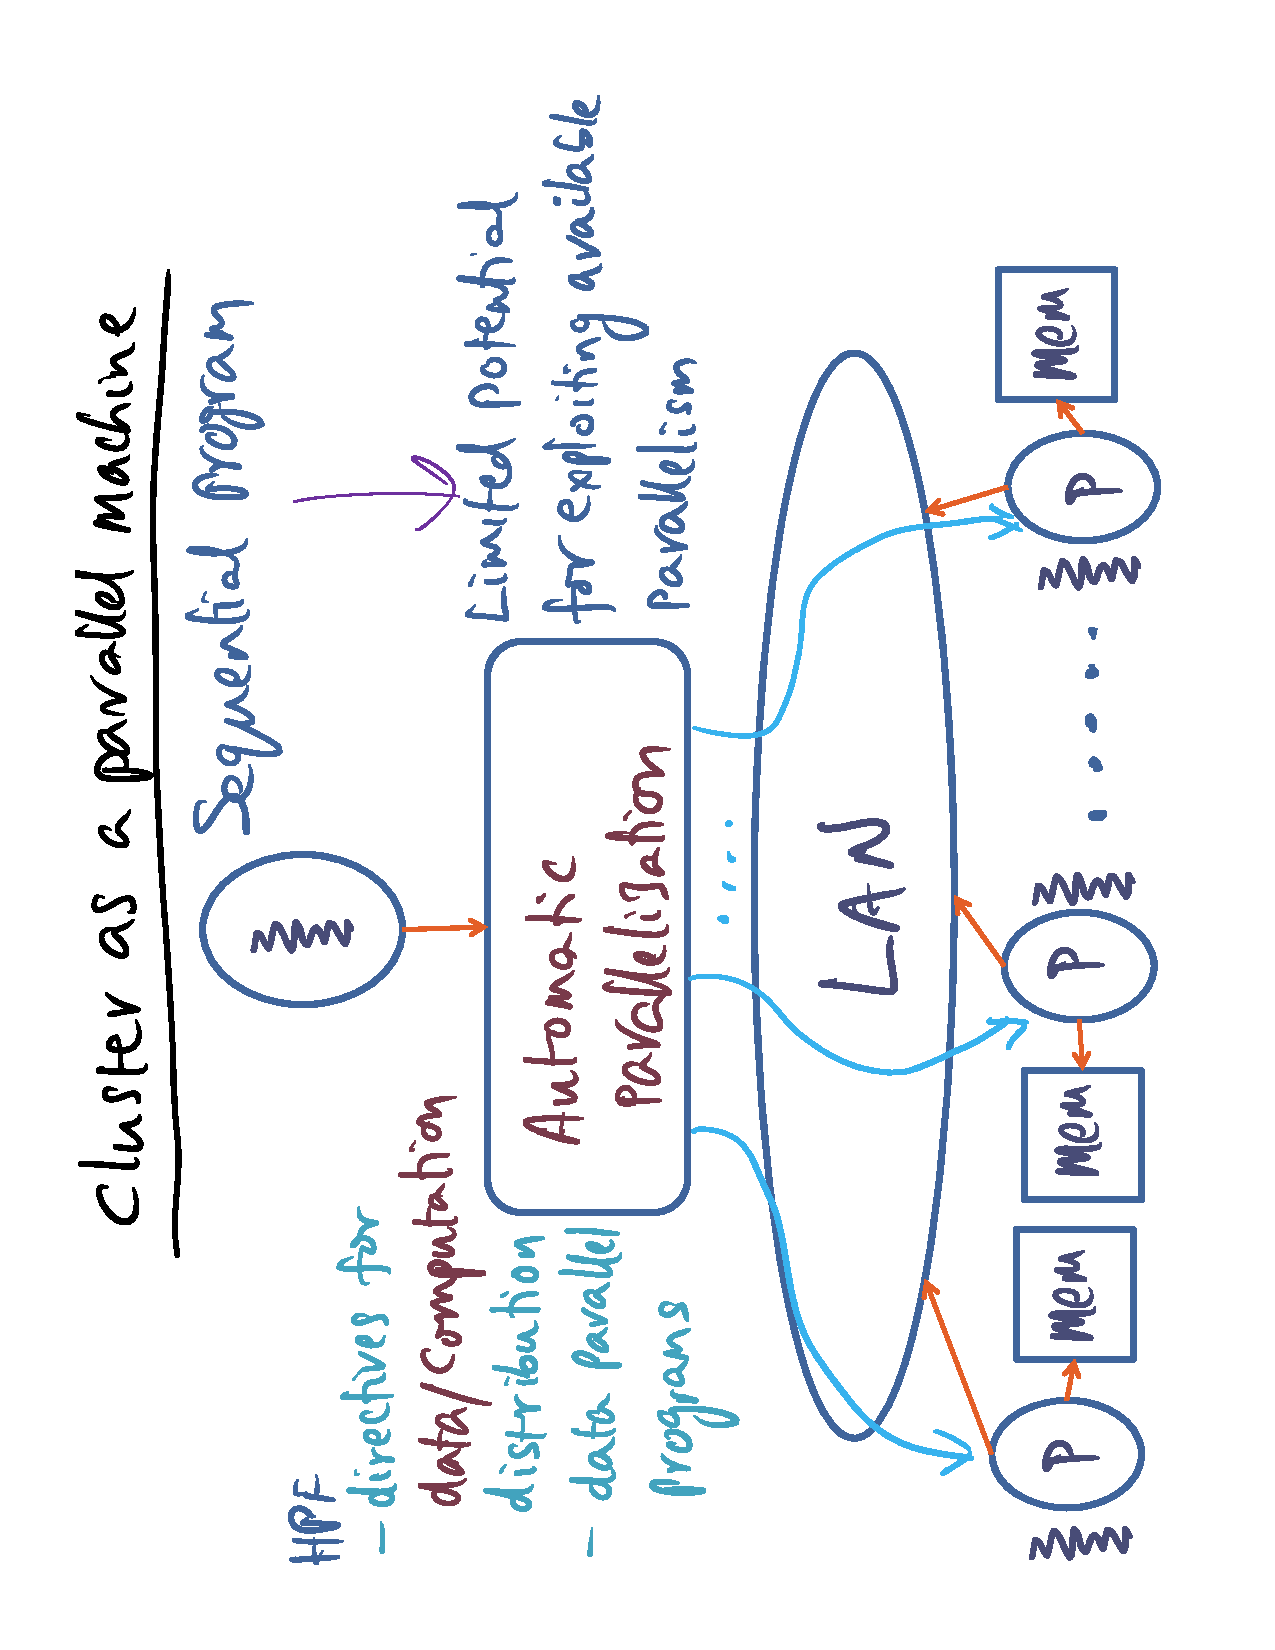
\includegraphics[width=\fullsize, angle=-90]{Figures/automatic-parallel-programming}
\caption{Automatic parallelization.}\label{fig: automatic-parallel}
\end{figure}

\noindent
{\bf Automatic Parallelization.} Assume that if the starting point is a sequential program. One possibility is to 
use so-called {\bf automatic parallelization}, an illustration of which is 
shown in~\autoref{fig: automatic-parallel}. 
That is, instead of writing an explicitly 
parallel program, we write a sequential program. And let somebody else do the heavy 
lifting in terms of identifying opportunities for parallelism that exits in the program 
and map it to the underlying cluster. That is called an implicitly parallel program. There 
are opportunities for parallelism, but the program itself is not written as a parallel 
program. Now it is the onus of the tool, in this case, an automatic parallelizing compiler, 
to look at the sequential program and identify opportunities for parallelism and exploit that by 
using the resources that are available in the cluster. High-performance FORTRAN is 
an example of a programming language that does automatic parallelization, but it is 
user-assisted parallelization in the sense that the user who is writing the sequential 
program is using directives for distribution of data and computation. And those directives are 
then used by this parallelizing compiler for mapping these computations onto the resources of 
a cluster. So it puts it on different nodes on the cluster and that way, it exploits the parallelism 
that is there in the hardware, starting from the sequential and doing the heavy lifting in terms 
of converting the sequential program to a parallel program to extract performance for this 
application. This kind of automatic parallelization, or implicitly parallel programming, works 
really well for certain classes of program called data parallel programs. In such programs, for this most 
part, the data accesses are fairly static, and it is determinable at the compile time. So in other words, there is limited potential for exploiting the available parallelism in the cluster if we resort to implicitly parallel 
programming. 

\begin{figure}
\centering
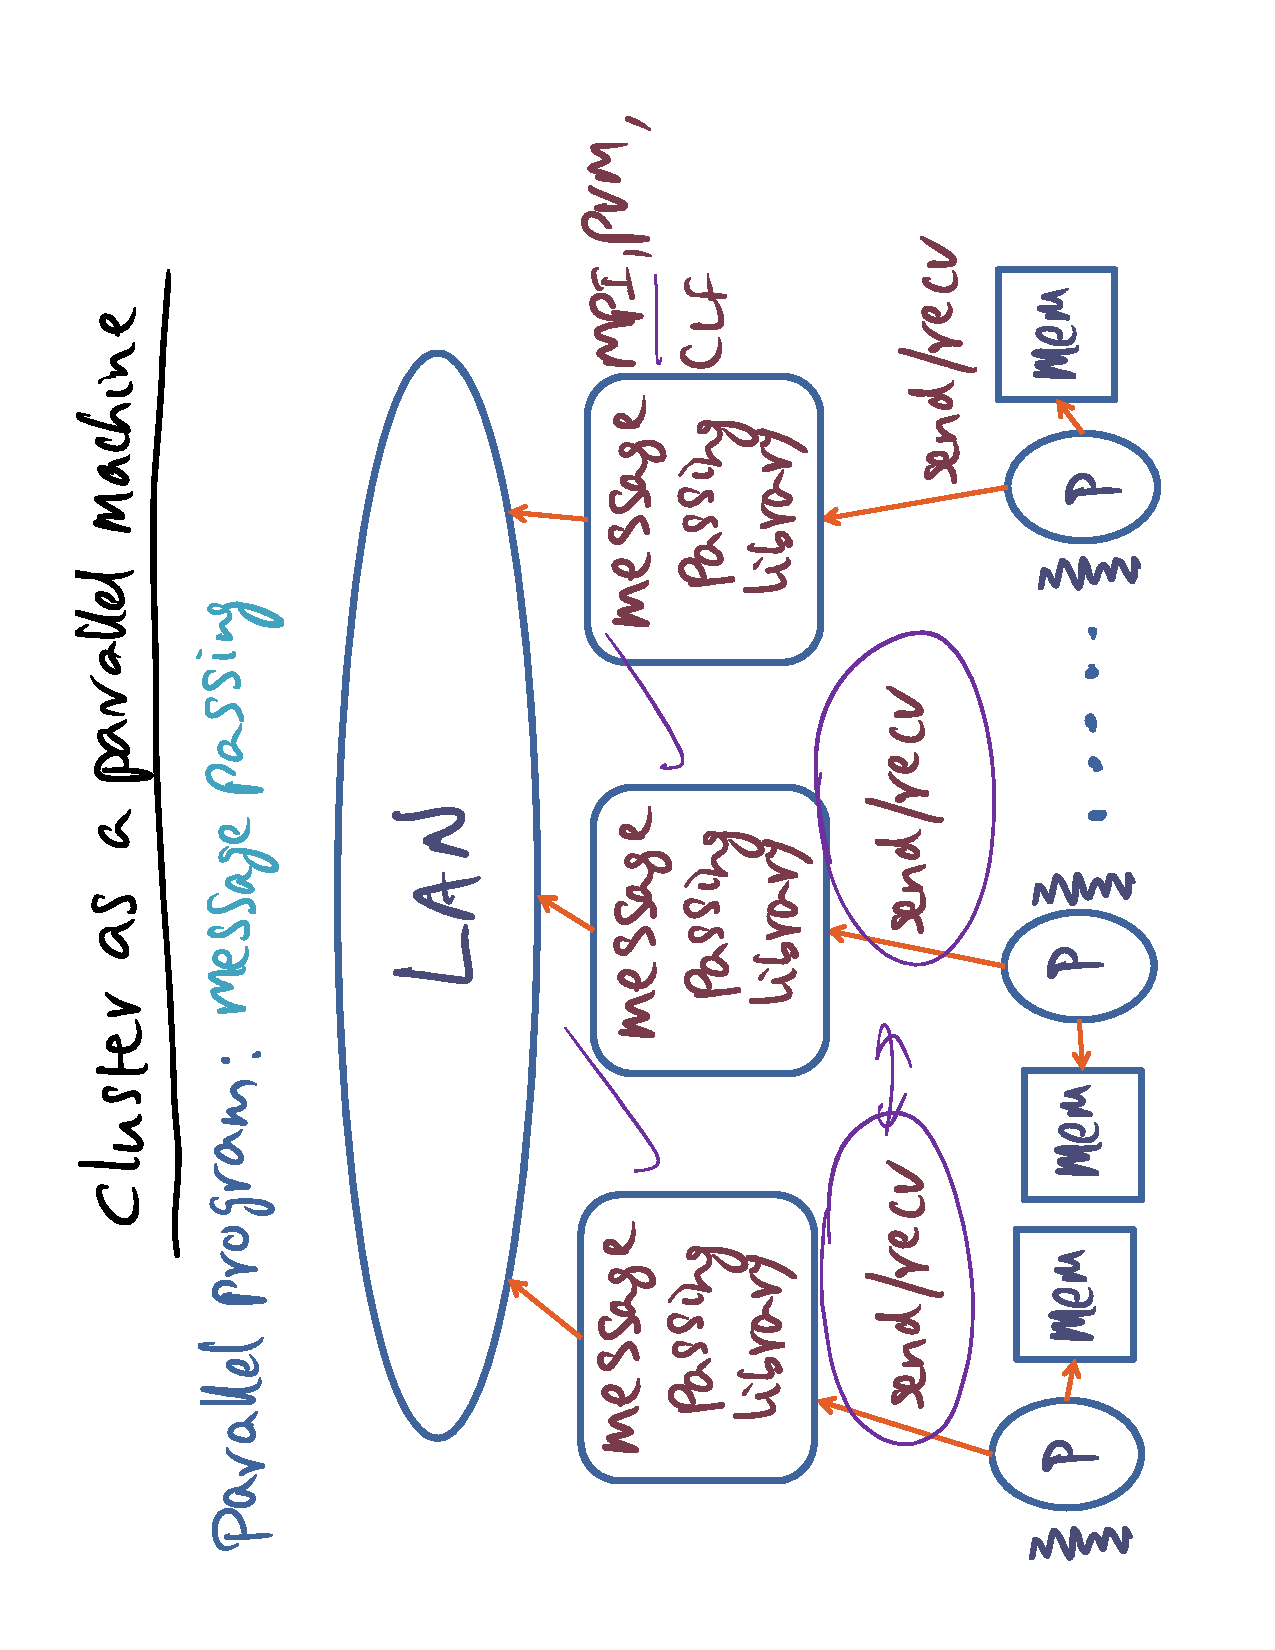
\includegraphics[width=\fullsize,angle=-90]{Figures/message-passing}
\caption{Message passing style of parallel programming.}\label{fig: message-passing}
\end{figure}

\noindent
{\bf Message Passing.} Therefore, we write the program as a truly parallel program instead of a implicitly parallel 
program. In other words, the application programmer is going to think about his/her application and write the 
program as an explicitly parallel program. And there are two styles of writing explicitly programs. And correspondingly 
system support for those two styles of explicitly parallel programs. One is called {\bf message passing} style of explicitly 
parallel program. The run time system is going to provide a message passing library which has primitives for 
an application thread to do sends and receives to its peers that are executing on other nodes of the cluster. 
\autoref{fig: message-passing} gives an illustration of message passing style of explicitly parallel program. 
So this message passing style of explicitly parallel program is true to the physical nature of the cluster. 
The physical nature of the cluster is the fact that {\it every processor have its private memory 
and this memory is not shared across all the processors.} So the only way a processor can communicate with 
another processor is by sending a message through the network from which one processor can receive messages.  
The processor can not directly reach into the memory of the other processor because that is not the way the cluster 
is architected. So the message passing library is true to the physical nature of the cluster that 
there is no physically shared memory. And there are lots of examples of message passing libraries that have been 
written to support explicitly parallel programming in a cluster, such as message passing interface (MPI), 
Parallel Virtual Machine (PVM)~\cite{pvm}, CLF~\cite{watkins2003clf}. And to this day, many scientific applications running on large-scale clusters in National Labs like 
Lawrence Livermore and Argonne National Labs and so on use this style of programming, using MPI as the 
message passing fabric. The only downside to the message passing style of programming is that it is difficult to 
program using this style. If you are a programmer who writes sequential programs, the transition path to writing an explicitly 
parallel program is easier if there is the notion of shared memory because it is natural to think of 
shared data structures among different threads of an application and that is the reason making the transition from 
sequential programming to parallel programming using for instance the {\code pthread} library on an SMP is 
a fairly intuitive and easy pathway. On the other hand, if the programmer has to think in terms of 
coordinating the activities on different processors by explicitly sending and receiving messages from 
the peers that is calling for a fairly radical change of thinking in terms of how to structure a 
program. 

\begin{figure}
\centering
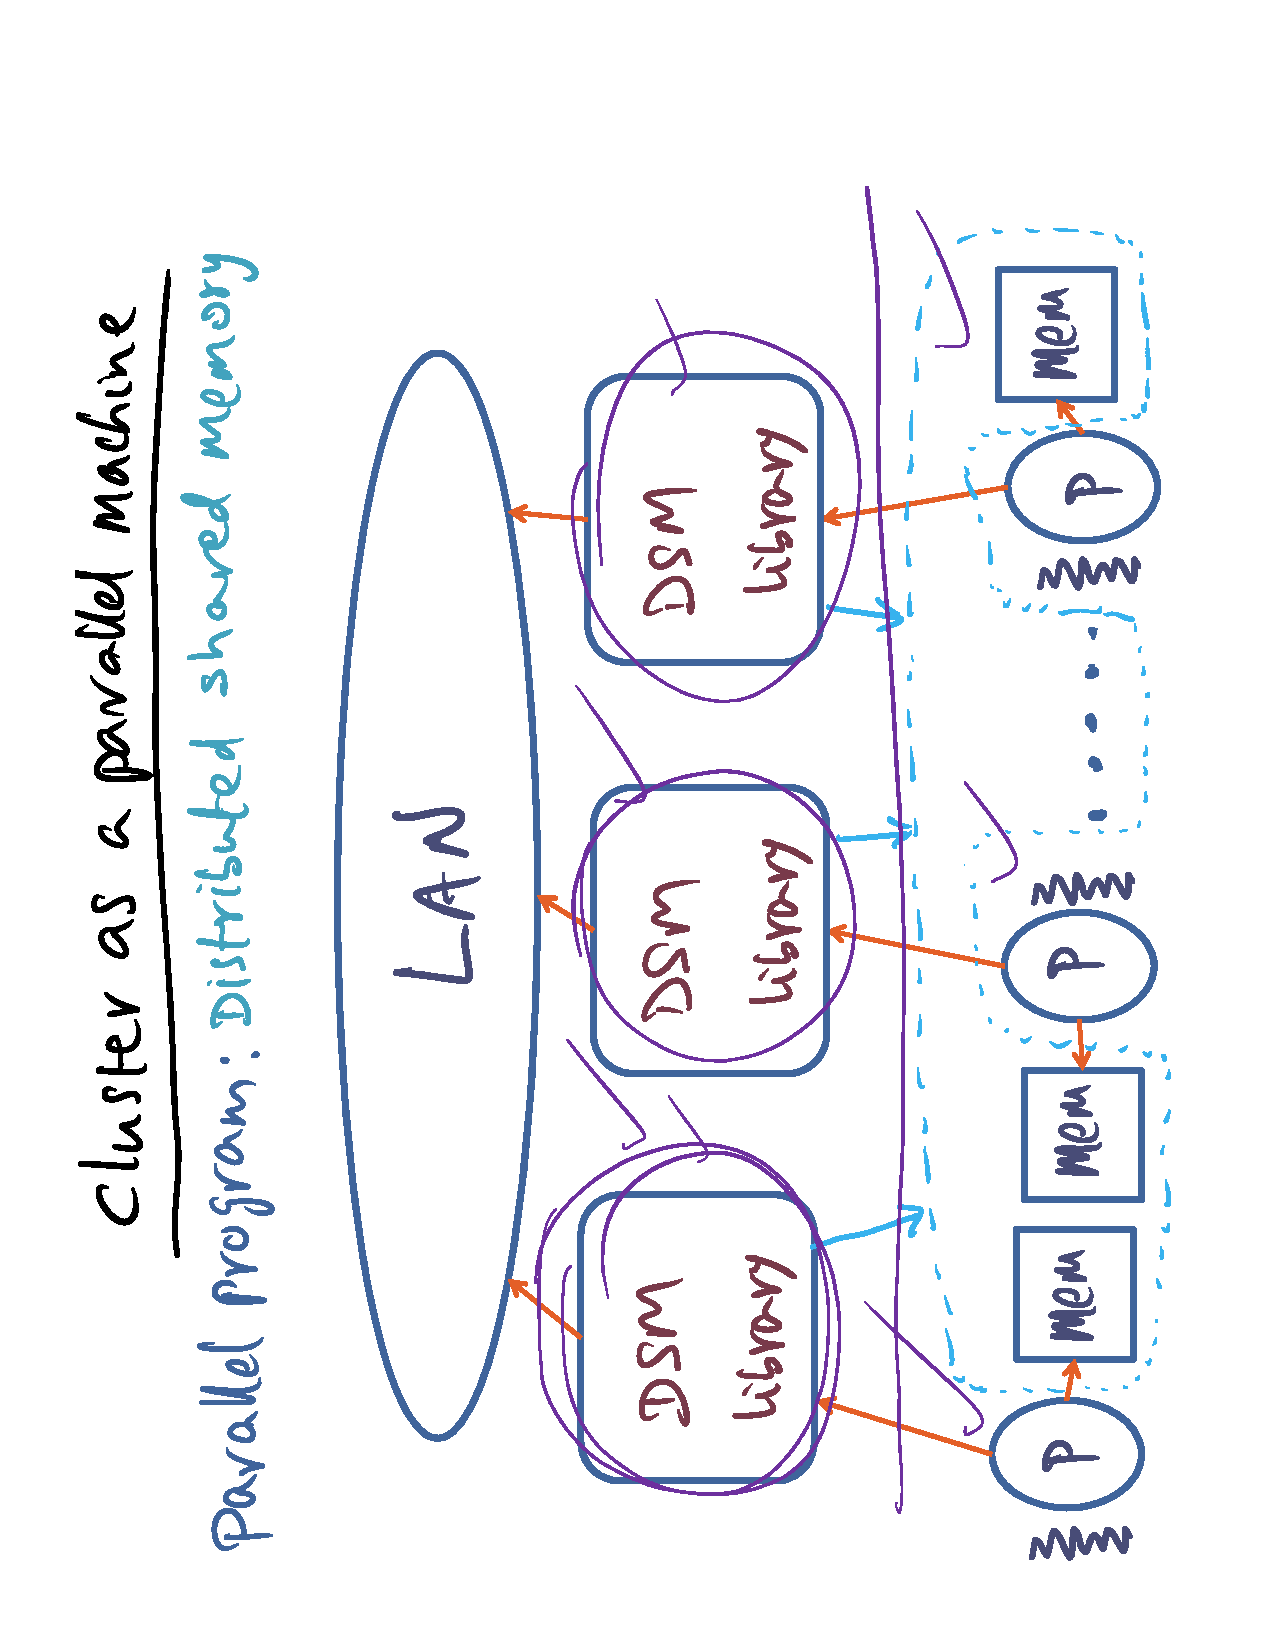
\includegraphics[width=\fullsize,angle=-90]{Figures/distributed-shared-memory}
\caption{DSM style of parallel programming.}\label{fig: distributed-shared-memory}
\end{figure}

\noindent
{\bf Distributed Shared Memory.} That is the motivation for coming up this abstraction of distributed shared memory 
in a cluster. The idea is that we want to give the illusion to the application programmer writing an explicitly 
parallel program that all of the memory in the entire cluster is shared. They are not physically shared, but the DSM library is going to give the illusion to the threads running on each of these processors that all of the memory 
is shared. Thus, they will have an easier transition path for instance from 
a sequential program or going from a program that they write on an SMP to 
a program that runs on a cluster because they do not have to think in terms of 
message passing but they think in terms of shared memory. Also since 
we have provided shared memory semantics in DSM, there is no need for 
marshaling and unmarshaling arguments that are being passed from one 
processor to another and so on all of that is being handled by the fact 
there is ``shared memory''. So when you make a procedure call and that 
 procedure call is touching some portion of memory that happens to be on 
 remote memory. That memory is going to magically become available 
 to the thread that is making that procedure call. In other words, 
 the DSM abstraction gives the same level of comfort to a programmer who is 
 used to programming a truly shared memory machine when they move to a cluster 
 because they can use the same set of primitives like locks and barriers for synchronization and the {\code pthread} style of creating threads that 
 will run on different nodes of the cluster and that's the advantage of the 
 DSM style of writing an explicitly parallel program. 

\begin{figure}
\begin{minipage}{\textwidth}
\centering
\begin{chronology}{1980}{2017}{0.9\textwidth}
\event[1983]{1988}{\begin{tabular}{c}BBN Butterfly~\cite{Alherbish1994BBN}\\ Sequent Symmetry~\cite{Graunke1990Sequent}\end{tabular}}
\event{1990}{KSR-1~\cite{Ramachandran1993ksr-1}}
\event[1992]{1994}{\begin{tabular}{c}Alewife~\cite{Agarwal1991alewife}\\ DASH~\cite{Lenoski1992DASH}\end{tabular}}
\event{1995}{SGI 2000~\cite{sgi2000}}
\event[2001]{2004}{SGI Altix~\cite{sgi-altix}}
\event[2006]{2007}{IBM Blue gene~\cite{ibm-bluegene}}
\event[2011]{2013}{Clusters of SMPs~\cite{cluster-of-SMPs}}
\end{chronology}
\caption{History of hardware shared memory systems.}\label{fig: hardware-dsm}
\end{minipage}%
\vspace*{1pt}
\begin{minipage}{\textwidth}
\centering
\begin{chronology}{1980}{2017}{0.9\textwidth}
\event[1983]{1988}{\begin{tabular}{c}
IVY~\cite{ivy}\\CLOUDS~\cite{clouds}\\Mirage~\cite{mirage}\\Mether~\cite{mether}
\end{tabular}}
\event[1991]{1992}{\begin{tabular}{c}
Munin~\cite{munin}\\Treadmarks~\cite{Amza1996DSM}
\end{tabular}}
\event[1996]{1998}{\begin{tabular}{c}
Blizzard~\cite{blizzard}\\Shasta~\cite{shasta}\\cashmere~\cite{cashmere}\\Beehive~\cite{beehive}
\end{tabular}}
\end{chronology}
\caption{History of software DSM systems.}\label{fig: software-dsm}
\end{minipage}%
\vspace*{1pt}
\begin{minipage}{\textwidth}
\centering
\begin{chronology}{1980}{2017}{0.9\textwidth}
\event[1991]{1994}{\begin{tabular}{c}
Linda~\cite{linda}\\Orca~\cite{bal1992orca}
\end{tabular}}
\event[1999]{2001}{Stampede~\cite{nikhil1998stampede}}
\event[2007]{2008}{\begin{tabular}{c}Stampede RT~\cite{stampedert}\\ PTS~\cite{Hilley2000PTS}\end{tabular}}
\end{chronology}
\caption{History of structured DSM systems.}\label{fig: structred-dsm}
\end{minipage}%
\end{figure}

\section{History of Distributed Shared Memory Systems}\label{sec: dsm-histroy}

Before going into details of DSM, let us first learn some history 
of the DSM systems. 
\autoref{fig: hardware-dsm}, \autoref{fig: software-dsm}, and \autoref{fig: structred-dsm} give the history of hardware, software and structured 
distributed shared memory in the past 20 years, respectively. Note that, these figures 
only gave the approximate time of when these systems were invented. 
If you are interested in more details of the history of DSM systems, 
the survey in~
\cite{Nitzberg1991survey} may be a good starting point.


\section{Implementation of DSM}\label{sec: impl-dsm}
\subsection{Shared Memory Programming: Revisit}\label{sec: smp}

In previous lectures, we have already learned the shared memory synchronization. {\bf Lock} is a primitive and particularly the 
mutual exclusion lock is a primitive that is used ubiquitously 
in writing shared memory parallel programs to protect data structure 
so that one thread can exclusively modify the data and release the 
lock so that another thread can inspect the data later on. And similarly 
{\bf barrier} synchronization is another synchronization primitive 
that is very popular in scientific programs. 

In particularly, if you are writing a shared memory program, there are 
two types of memory accesses. One type of memory access is the normal reads 
and writes to shared data that is being manipulated by a particular thread. The second kind of memory access is for synchronization variables that are 
used in implementing locks and barriers by the operating system itself. It 
may be the operating system or it could be a user level threads library that 
is providing these mutual exclusion locks, or barriers primitives, but in implementing those synchronization primitives, those algorithms are going to 
use reads and writes to shared memory. 


\begin{figure}
\centering
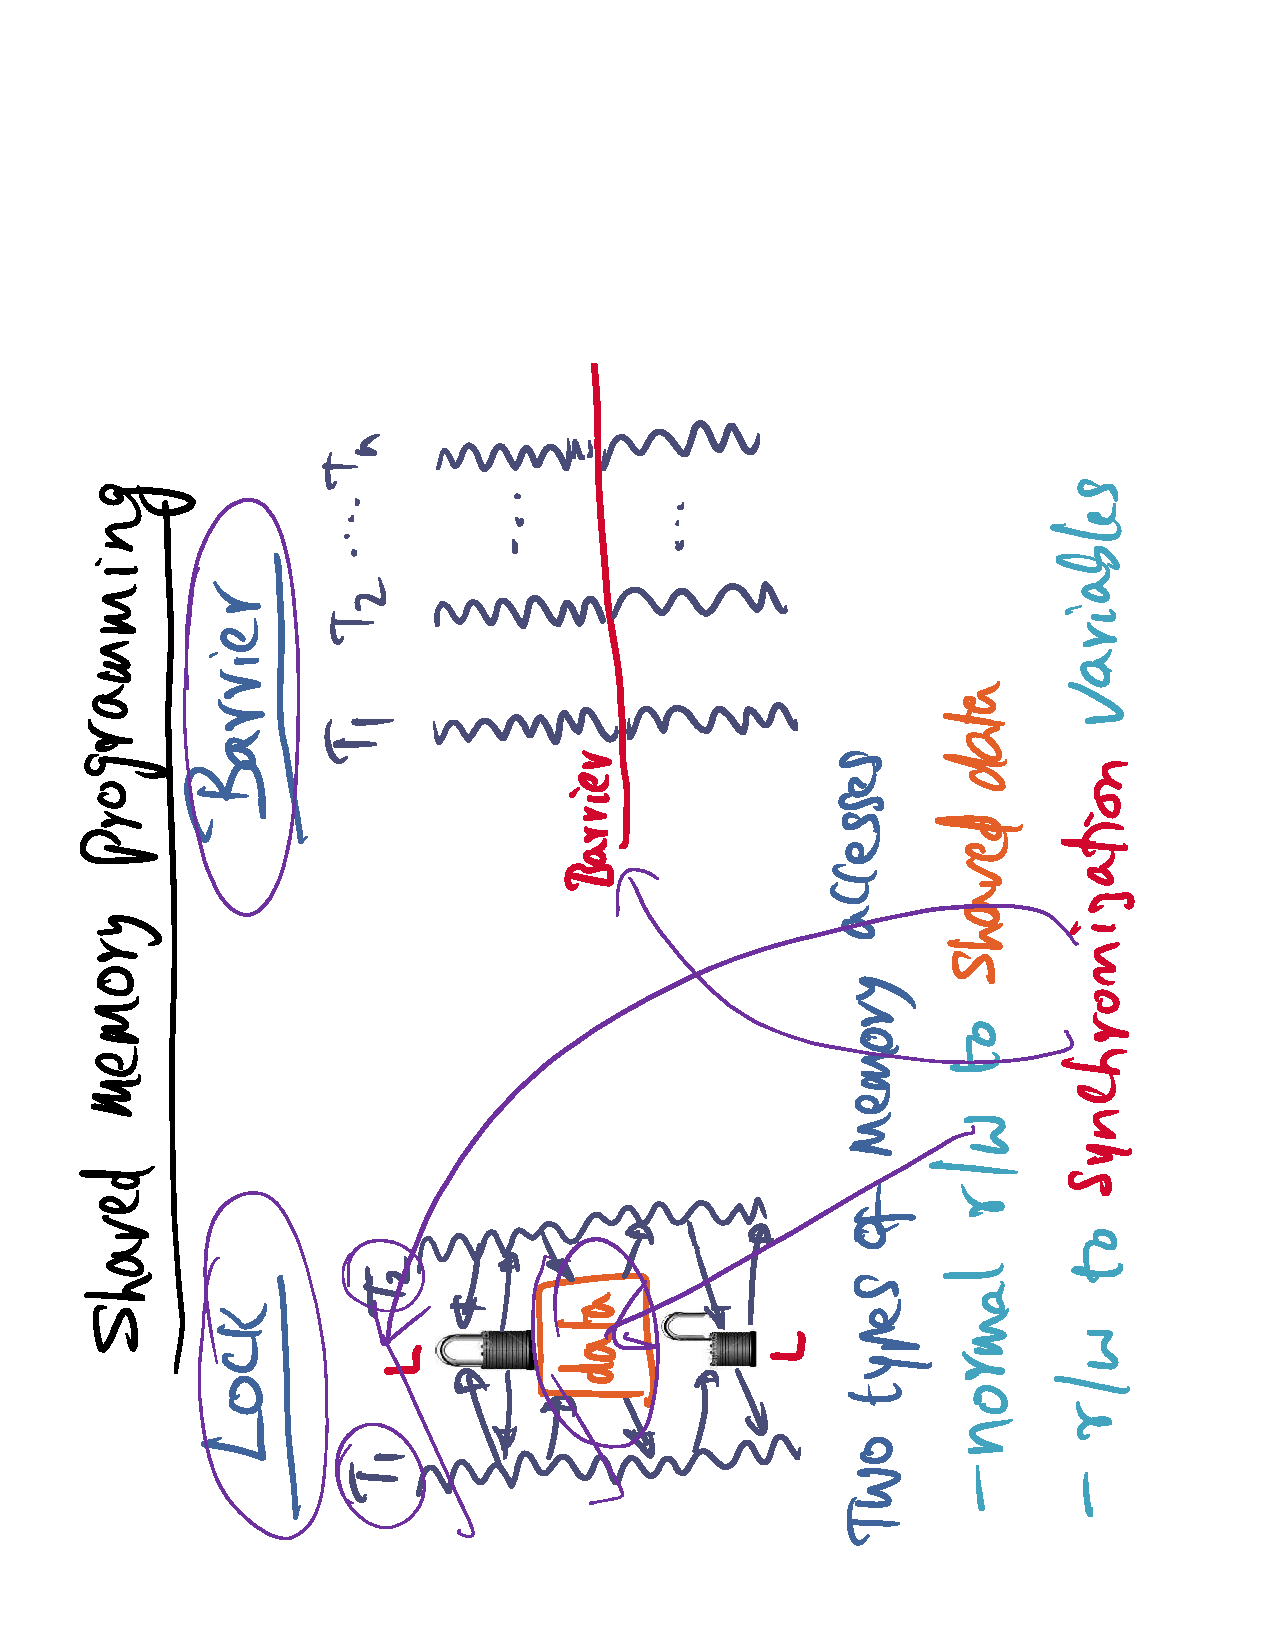
\includegraphics[width=\fullsize,angle=-90]{Figures/smp}
\caption{Shared memory synchronization.}\label{fig: smp}
\end{figure}

\subsection{Memory Consistency}\label{subsec: mem-consistency}

Recall that, in previous lectures, we have discussed the relationship between the 
memory consistency model and cache coherence, in the context of shared memory systems. 
Memory consistency model is a contract between the application programmer and the 
system. It answers the {\bf when} question, that is, when a shared memory location 
is modified by one processor, when ({\it i.e.,} how soon) that change is going to be made 
visible to other processors that have the same memory location in their respective 
caches. Cache coherence, on the other hand, is answering the {\bf how} question, 
that is, how is the system\footnote{Note that, by system, we actually mean the system software plus the hardware working together.}, 
implementing the contract of the memory consistency model ? In other words, the 
guarantee that is made by the memory consistency model, to the application 
programmer has to be fulfilled by the cache coherence mechanism. 

Now, coming back to writing a parallel program, when accesses are made to the shared 
memory, the underlying coherence mechanism has to ensure that all the processors 
see the changes that are being made to shared memory, commensurate with the 
memory consistency model. 

\begin{figure}
\centering
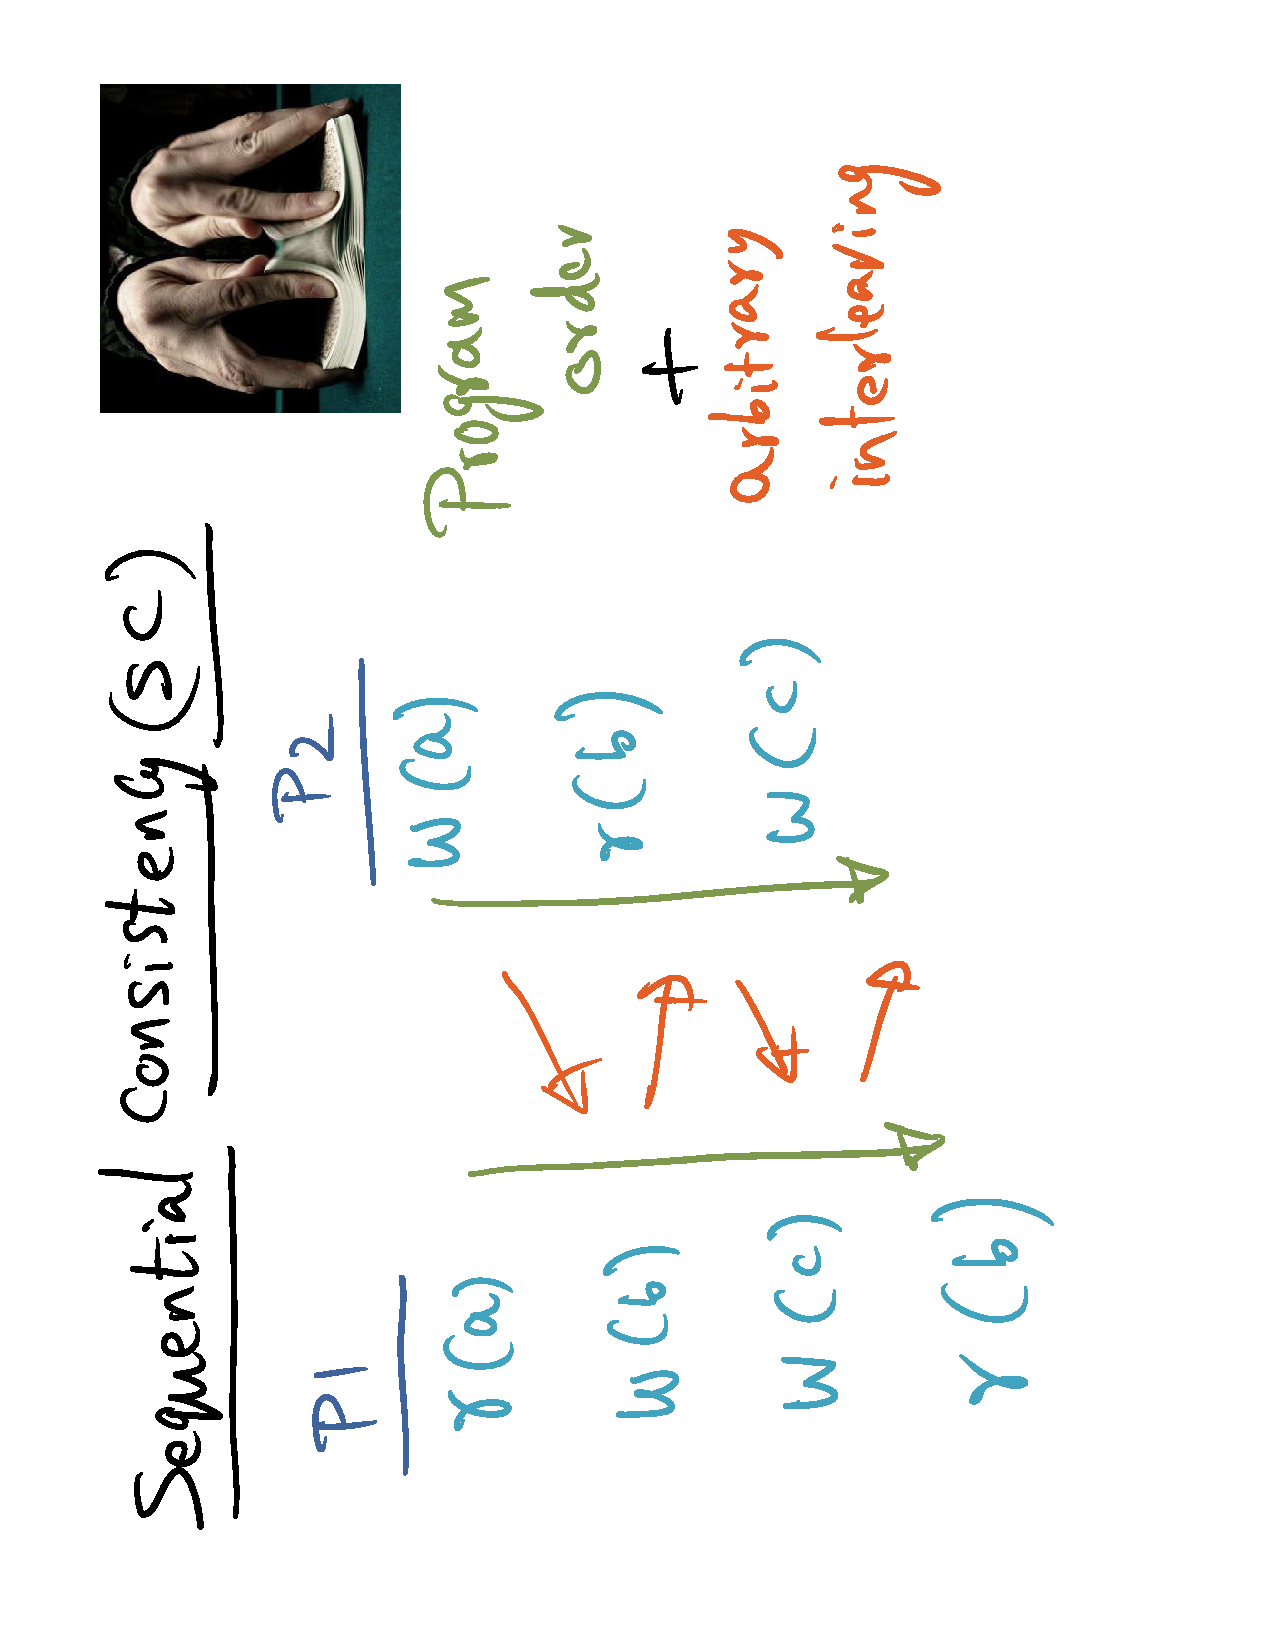
\includegraphics[width=\fullsize,angle=-90]{Figures/sc}
\caption{Sequential consistency.}\label{fig: sc}
\end{figure}

\noindent
{\bf Sequential Consistency (SC).} One particular memory consistency model that we have discussed 
in previous lectures is the sequential consistency. The idea behind sequential consistency is 
very simple. That is, every process is making some memory accesses. For example, as shown 
in~\autoref{fig: sc}, Process $P1$ have $4$ memory accesses. From the perspective of 
the programmer, the expectation is that, these memory accesses are happening in the textual order 
({\it i.e.,} {\code read(a)} $\rightarrow$ {\code write(b)} $\rightarrow$ {\code write(c)} $\rightarrow$ {\code read(b)}). Similarly, the expectation of the memory accesses of Process $P2$ 
is that {\code write(a)}$\rightarrow$ {\code read(b)} $\rightarrow$ {\code write(c)}. The real 
question is what happens to the accesses that are happening on one processor with respect 
to the accesses on another processor if they are accessing exactly the same memory location ? 
For instance, Process $P1$ is reading location {\code a}, and Process $P2$ is writing location 
{\code a}. What is the order between this read by $P1$ and this write by $P2$ ? That is 
where sequential consistency model says that the interleaving of memory accesses between 
multiple processors (\autoref{fig: sc} is showing two, but you can have arbitrary number of 
those processors) making accesses to shared memory all in parallel. When that happens 
you want to observe the textual program order for the accesses in an individual processor 
but the interleaving of the memory accesses coming from the different processors is 
arbitrary. In other words, the sequential memory consistency model builds on the atomicity 
for individual read/write operations and says that, individual read/write operations 
are atomic on any given processor, and the program order has to be preserved. And, in order to think 
about interleaving of the memory accesses that are happening on different processors. That can be 
arbitrary and should be consistent with the thinking of the programmer. 

Back to our parallel program. As shown in~\autoref{fig: sc-upshot}, a parallel program is making read/write 
accesses to shared memory, some of them offer data, some of them offer synchronization. Now, 
as far as the sequentially consistent memory model is concerned, it does not distinguish 
between accesses coming from processors as data accesses, or synchronization accesses. So there 
will be coherence action on every read/write access that the model sees. For example, 
if $P1$ (in~\autoref{fig: sc-upshot}) writes to a memory location, then the sequentially consistent memory model 
has to ensure that this write is inserted into the global order somewhere. However, to 
insert into the global order somewhere, it has to perform the coherence action with respect to all 
the other processors. That is the upshot of not distinguishing between normal data accesses 
and synchronization accesses that is inherent in the SC memory model. 

\begin{figure}
\centering
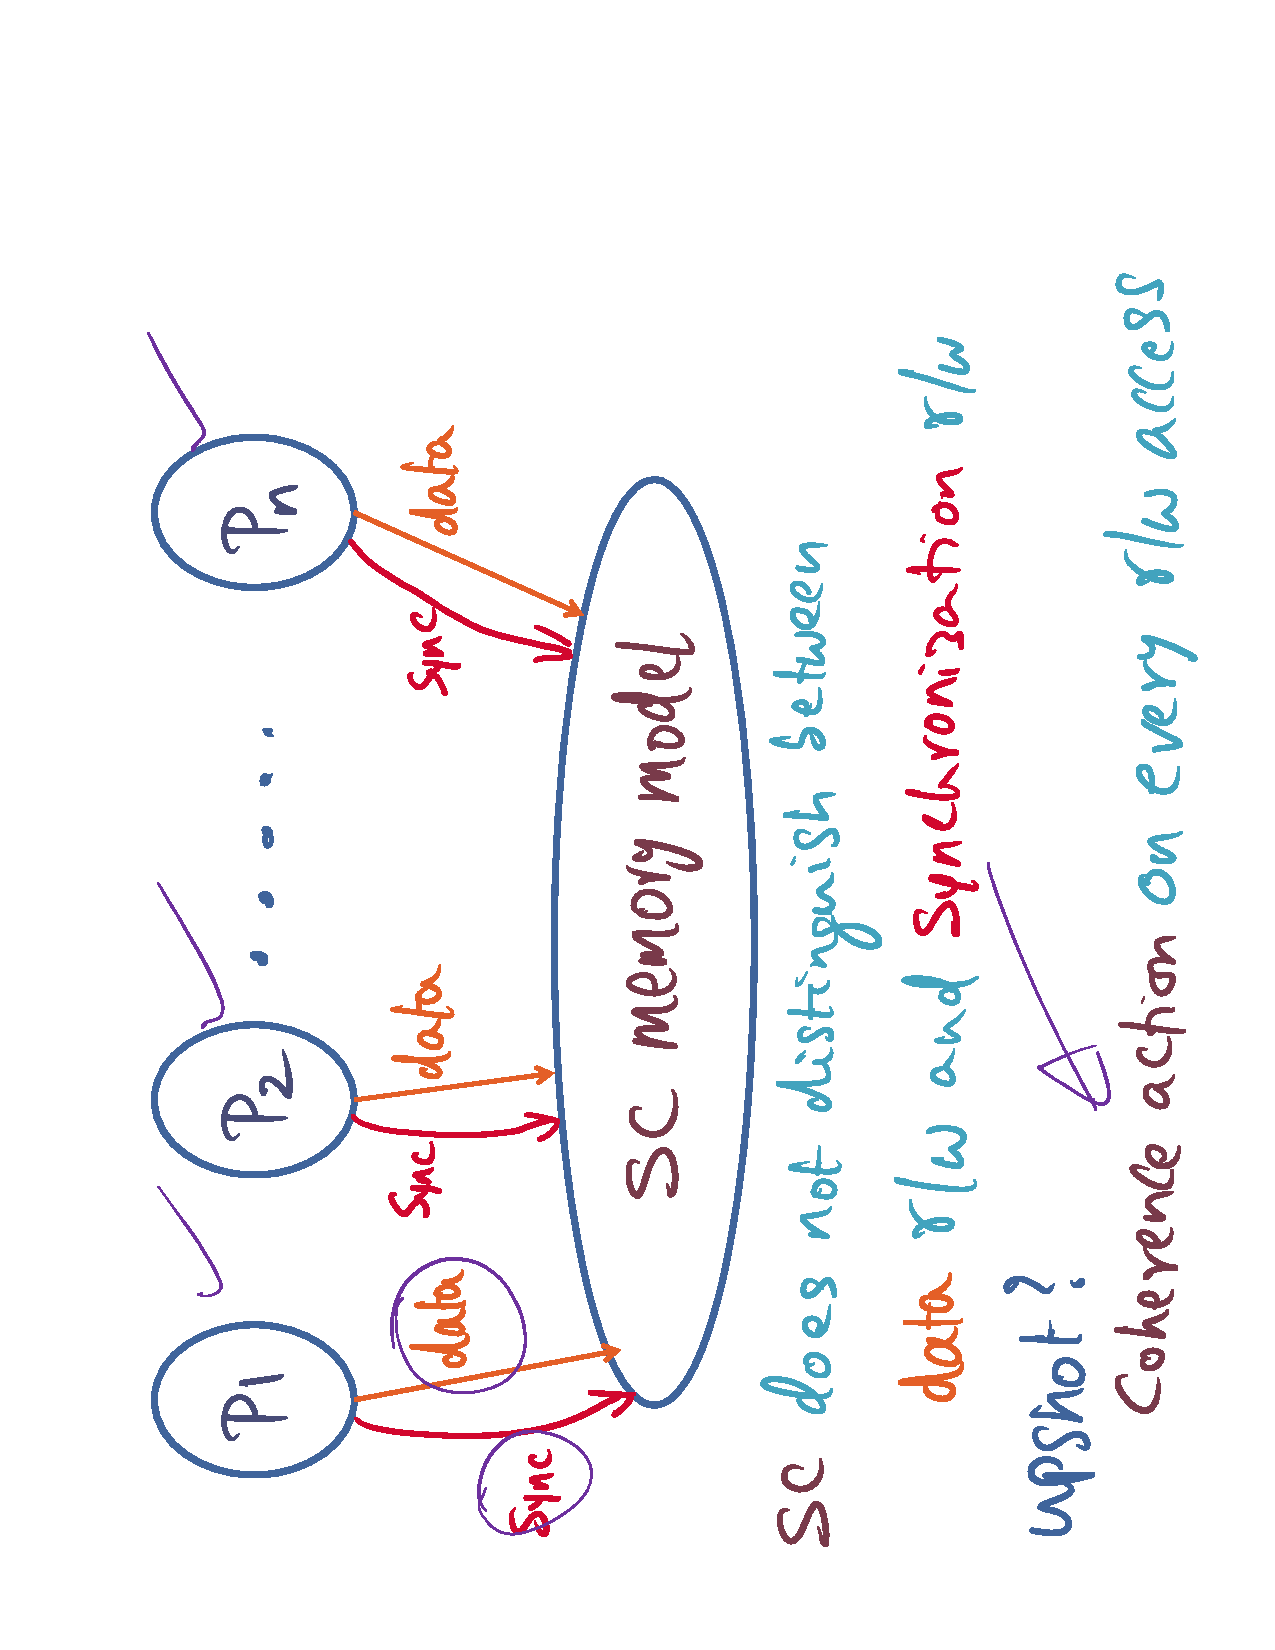
\includegraphics[width=\fullsize,angle=-90]{Figures/upshot-sc}
\caption{Illustration of sequential consistency in a parallel program.}\label{fig: sc-upshot}
\end{figure}

Now, let us see a typical parallel program shown in~\autoref{fig: typical-parallel-program}. 
In the program, we decided that 
the accesses to shared variables {\code a} and {\code b} should be governed by a lock 
{\code L}. So if any process wants to read or write variables {\code a} and {\code b}, it will get a lock 
and then mess with variables that are governed by this lock. Once the process is done with whatever 
it wants to do with 
these shared variables, it will unlock indicating that it is done. And the codes between 
{\code Lock(L)} and {\code Unlock(L)} are the critical section. Within the critical section, 
processes are allowed to do whatever they want on these data structures that are governed by this particular lock, 
because that is an association we as the programmer have made in writing the parallel program. So if another process 
say $P2$, gets the same lock. It is going to get the lock only after $P1$ has released it. And consequently, 
if you look at the structure of the critical section of $P2$, it gets a lock and it is messing 
with the same data structures that $P1$ was messing with in its critical section. But, by design, we know 
that either $P1$ or $P2$ can be messing with the data structures at any point of time. And that is a 
guarantee that we know comes from the fact that we designed the parallel program. And the lock is associated with these data 
structures. So in other words, $P2$ is not going to access any of the data that is inside the critical section until $P1$ 
releases the lock. We know this because we design the program, but the SC memory model does not know 
about the association between these data structures and the lock. And in particular, it does not 
even know that memory access emanating from the processor due to the lock primitive is a ``different animal'' 
compared to the memory accesses coming from the processor as a results of accessing normal data 
structures. So the cache coherence mechanism that is provided by the system for implementing the 
memory consistency model is going to be doing more work that it needs to do because it is going to take actions on every 
one of these accesses, even though the coherence actions are not warranted for these data in the critical section 
of $P1$ until $P1$ releases the lock. So what that means is that there is going to be more overhead for 
maintaining the coherence commensurate with the SC memory model. That means it is going to lead to a pooler 
scalability of the shared memory system. So in this particular example, since $P2$ is not going to access any 
of these data structures in its critical section until $P1$ has released the lock. There is no need for 
coherence action for {\code a} and {\code b} until the lock is actually released. 

\begin{figure}
\centering
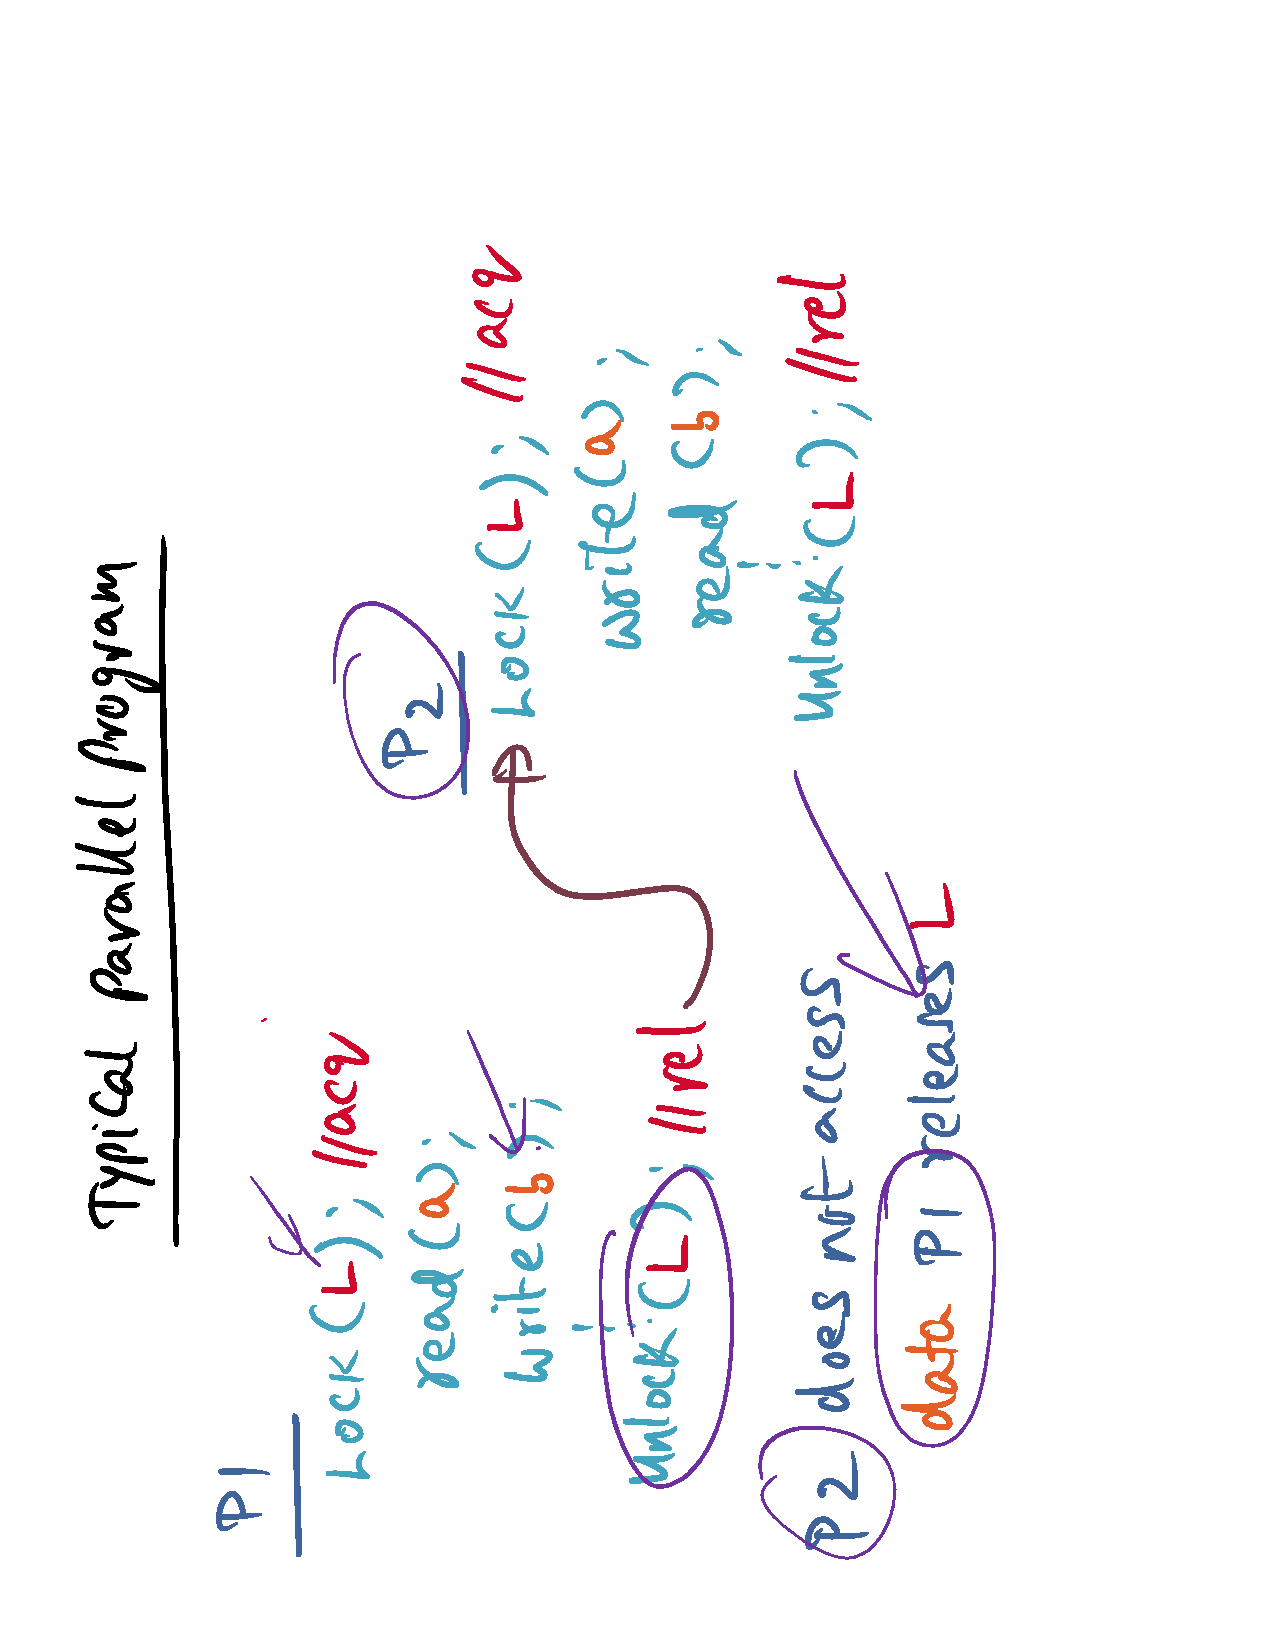
\includegraphics[width=\fullsize,angle=-90]{Figures/typical-parallel-program}
\caption{A typical parallel program.}\label{fig: typical-parallel-program}
\end{figure}

\noindent
{\bf Release Consistency (RC).} This is the motivation for another memory consistency model, which is called 
release consistency. Generally, the parallel program consists of several different parallel threads 
({\it e.g.,} $P1$ and $P2$ in ~\autoref{fig: rc}), and if any process (or thread) wants to mess with some shared data 
structures, it is going to acquire a lock ({\it e.g.,} $a1$ in~\autoref{fig: rc}) and in the mind of the programmer 
there is an association between this lock and the data structures governed by it. So long as they hold 
the lock they can modify the data structure and then release the lock ({\it e.g.,} $r1$ in~\autoref{fig: rc}). So 
every critical section you can think of as composed of an acquire followed by data accesses governed 
by the lock and then a release. If the same lock is used by some other process ({\it e.g.,} $P2$) and 
if the critical section of $P1$ preceded that of $P2$. In other words, $r1$ of $P1$ happens before 
$a2$ of $P2$. If this acquire operation for the same lock happened after the release of that lock. 
All that we have to ensure is that all the coherence actions prior to this 
release of the lock by $P1$ has to be complete before we allow $P2$ to acquire this lock. That is 
the idea of release consistency. So we take the synchronization operations that are provided 
by the system whether it is hardware or software and we label them as either an acquire operation 
or a release operation. So it is very straightforward when you think about mutual exclusion lock 
where the lock primitive is the acquire operation, while the unlock primitive is the release 
operation. Other synchronization operations can also be mapped to acquire and release, for example, 
the barrier synchronization. The arrival of a barrier is equivalent to an acquire and leaving the 
barrier is equivalent to a release. 

Therefore, if $P1$ does a shared memory access within its critical section, and that shared memory access 
would normally result in some coherence actions on the interconnect reaching to the other processes 
and so on. If it is a SC memory model we will block process $P1$ until that particular memory access 
is complete with respect to all the processes in the shared memory machine. But if we use the release consistency 
model, we do not have to block $P1$ in order for coherence actions to be complete to let the process 
continue on with its computation. We only have to block a process at a release point to make 
sure that any coherence actions that may have been initiated up until the release point are all complete 
before we perform this release operation. So the RC model allows exploitation of computation on $P1$ 
with communication that may be happening through the coherence mechanism for completing the 
coherence actions corresponding to the memory accesses that are making inside the critical section. 

\begin{figure}
\centering
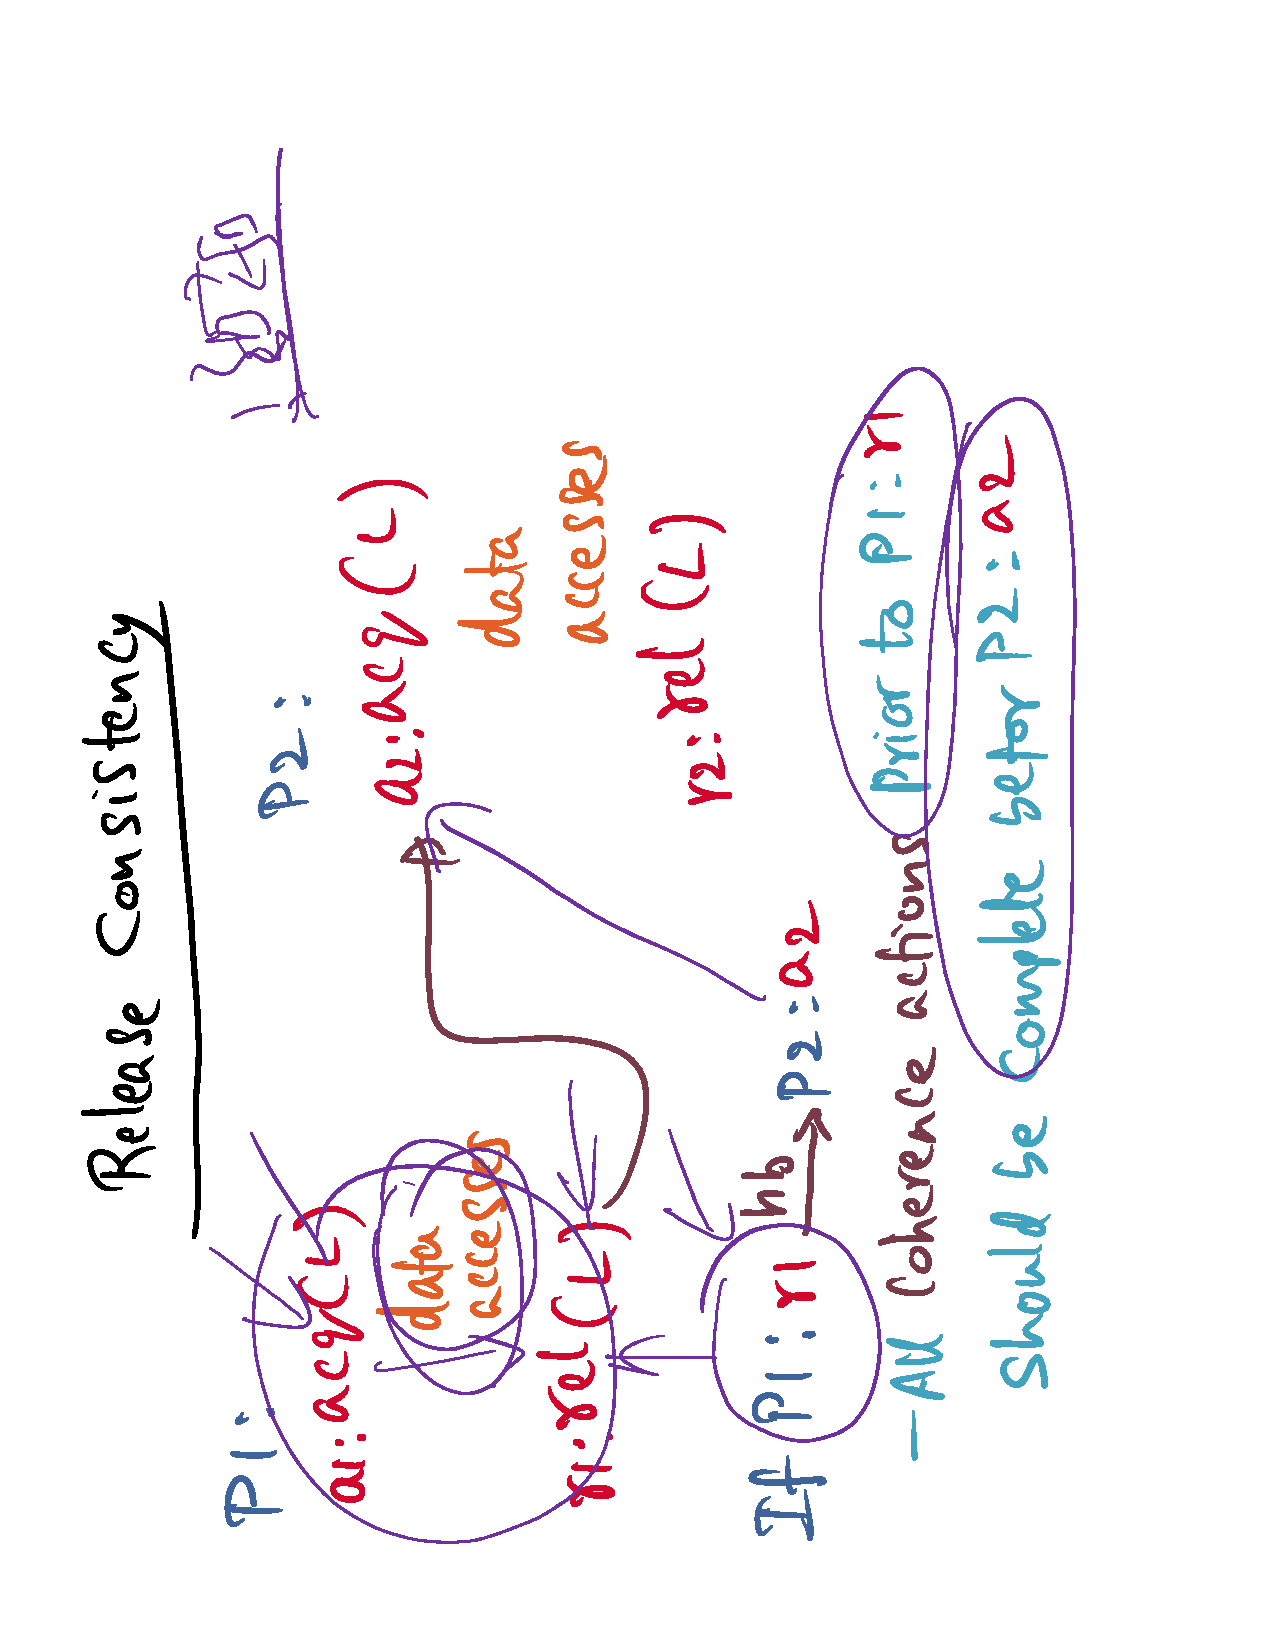
\includegraphics[width=\fullsize,angle=-90]{Figures/rc}
\caption{Release consistency.}\label{fig: rc}
\end{figure}

\noindent
{\bf Lazy RC.} Now, let us see a lazy version of the RC memory model. It is called LRC. \autoref{fig: rc} 
gives you the structure of a parallel program: a thread acquires a lock, does the data accesses, releases the 
lock; another thread may acquire the same lock. Recall that if the critical section of $P1$ precedes 
that of $P2$, then the RC memory model requires that, at the point of release ({\it i.e.,} $r1$),  
you ensure that all the modifications that have been made on processor $P1$ are all communicated to 
other processors through coherence actions. Then, $P1$ releases the lock. That is called {\bf 
eager release consistency}, meaning that at the point of release you are ensuring that the 
entire system is cache coherent at the point of release. Assume that $P2$'s acquire happens much 
later than $P1$'s release of the same lock. Clearly, there is an opportunity for 
procrastination. We have already seen that procrastination often helps in system design ({\it e.g.,} 
mutual exclusion locks and process scheduling) in previous lectures. So lazy RC is another instance 
where {\bf procrastination may actually help in optimizing the system performance}. The idea is that, 
rather than performing all the coherence actions at the point of release. But wait till the acquire 
actually happens. At the point of acquire, take all the coherence actions before allowing this acquire to succeed. 
So the key point is that you are deferring the point at which you ensure that all the coherence 
actions are complete to the point of acquisition as opposed to the point of release. 

\begin{figure}[!htbp]
\centering
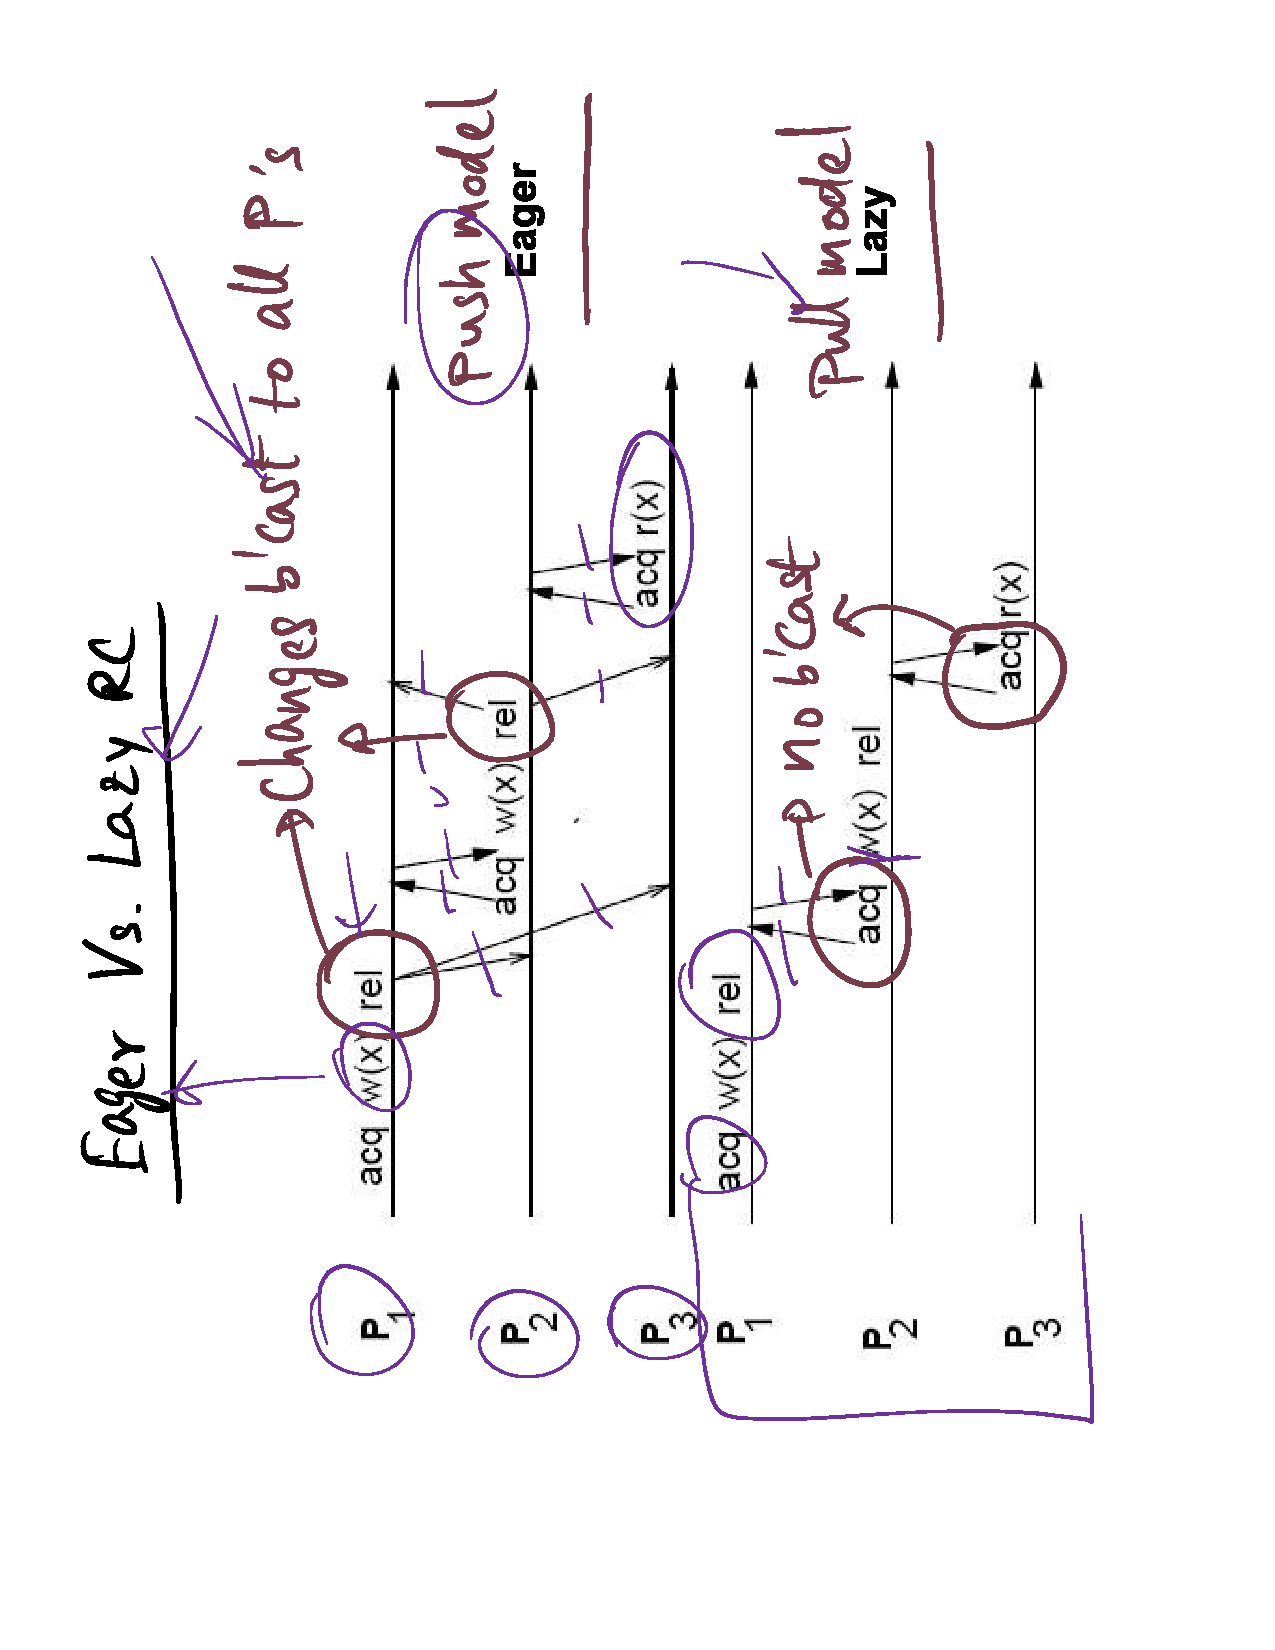
\includegraphics[width=\fullsize,angle=-90]{Figures/ERCvsLRC}
\caption{Eager RC vs. lazy RC.}\label{fig: lrc-vs-erc}
\end{figure}

\autoref{fig: lrc-vs-erc} gives the comparison between eager RC and lazy RC. As you can see, in the eager 
version of RC memory model, $P1$ has to communicate to all other processors to ensure that the 
changes on variable {\code x} are visible to them at the release point, and so does $P2$. Now move over to 
the lazy version. Note that, in the lazy version, we did nothing while $P1$ releases its lock, later on, 
the next processor that happens to acquire the same lock. The RC memory model 
has to make sure that all coherence actions associated with that particular lock have been complete. In this example, 
the previous lock holder, {\it i.e.,} $P1$, has made changes to variable {\code x}, so the RC memory model 
will pull it from $P1$, and then $P2$ can execute its critical section. Then, before $P3$ executes its critical 
section, it is going to pull it from $P2$, and complete what it needs to do. The most important thing 
that we need to pay attention to is that there is no broadcast anymore. There is only point-to-point 
communication that is happening between processors that are passing the lock from one to the other. Note that, 
lazy RC memory model is also called {\bf pull model}, since we are pulling the coherence actions at the point of acquisition. 
Whereas the eager version is called {\bf push model}. \autoref{tab: erc-vs-lrc} summarizes the pros and 
cons of the eager RC and lazy RC, respectively. 

\begin{table}
\centering
\caption{Eager RC vs. lazy RC.}\label{tab: erc-vs-lrc}
\begin{tabular}{@{}*{7}{c}}
\toprule 
\multicolumn{3}{c}{\bf Eager RC}&\phantom{ab}&\multicolumn{3}{c}{\bf Lazy RC}\\
\cmidrule(lr){1-3}\cmidrule(lr){5-7}
{\bf Pros} &\phantom{a}& {\bf Cons} && {\bf Pros} &\phantom{a}& {\bf Cons} \\
\midrule
Lower latency at acquisition&&More messages  && Less messages && More latency at acquisition\\
\bottomrule
\end{tabular}
\end{table}

\subsection{Software DSM}\label{subsec: softDSM}

So far, we have seen three types of memory consistency model: sequential consistency, eager release consistency, 
and lazy release consistency. Strictly specking, the latter two are just two different versions of the release 
consistency memory model. Now it is the time to take the transition to talking about {\bf software distributed 
shared memory} and we will see how these memory models are coming to play in building software distributed 
memory. 

Recall that, we are dealing with a computational cluster. In the cluster, each node has its own private physical 
memory, but there is no physically shared memory. Therefore, the system software has to implement the consistency model 
to the programmer. In a tightly coupled multiprocessor system, coherence is maintained at individual memory 
access level by the hardware. Unfortunately, that fine-grain coherence maintenance at individual memory access 
level will lead to too much overhead in a cluster. Why ? Because on every load or store instruction that 
is happening on any one of these processors, the system software has to butt in, and implement the coherence actions 
in software through the entire cluster. Clearly, that is infeasible. So what do we do to implement software DSM? 

The first thought is to implement this sharing and coherence maintenance at a much coarse level, for example, 
at the level of pages. Actually, in an individual processor, or shared memory multiprocessor system, the 
coherence maintenance is not simply a single word that a processor is doing a load or a store on. Because 
in order to exploit spatial locality, the block size used in caches in processors tend to be bigger than the 
granularity of memory access that is possible from individual instructions in the processor. Here we are going to do 
the coherence maintenance in software, and we keep the granularity of coherence maintenance to be an 
entire page. And we are going to maintain the coherence of the distributed shared memory in software by cooperating with 
the operating system that is running on every node. So what we are going to do is we are providing a global 
virtual memory abstraction to the application programmer running on the cluster. So the application programmer 
can view the entire cluster as a globally shared virtual memory system. Under the cover what the DSM software 
is doing is to partition the global address space into chunks that are managed individually on the nodes of the different 
processors of the cluster. From the application point of view, what this global virtual memory abstraction is 
giving is address equivalence and that is if I access a memory location, say {\code X} in the program 
that means exactly the same thing whether I access the memory location {\code X} from processor $1$ or 
processor $2$ and so on so forth. That is the idea in providing a global virtual memory abstraction. And 
the way the DSM software is going to handle maintenance of coherence is by having distributed ownership for 
the different virtual pages that constitute this global virtual address space. So you can think of the global 
virtual memory space as constituted by several pages. And we are going to say some number of pages are 
owned by processor $1$, some number of pages are owned by processor $2$, and so on so forth. That is 
we split the ownership responsibility into individual processors. What that means is that the owner of 
a particular page is also responsible for keeping complete coherence information for that particular page and 
taking the coherence actions commensurate with that page. And the local physical memory 
available in each processor is being used for hosting portions of the global virtual memory space 
in the individual processor commensurate with the access pattern that is being displayed by the application on the 
different processors. For instance, as shown in \autoref{fig: SDSM}, if processor $1$ accesses certain portion 
of the global virtual memory space, then this portion is mapped into the local physical memory of this processor. 
So that the thread that is running one this processor can access this portion of the global address space. 
And it might be that the same page is being shared with some other processor. In that case, a copy of this 
page is existing in both of the two processors. Now it is up to the processor that is responsible for the ownership 
of this particular page to worry about the consistency of this page that is now resident in multiple 
locations. For instance, if node $1$ ({\it i.e.,} $P1$) is the owner of this page, then node $1$ will have the metadata that 
indicates that this particular page currently shared by $P1$ and $PX$. That is the directory that is 
associated with the portion of the global virtual memory space that is being 
owned and managed by $P1$. So statically we make an association between a portion of the address space and 
the owner for that portion of the address space in terms of coherence maintenance for that portion of 
the global virtual memory space. 

\begin{figure}[!htbp]
\centering
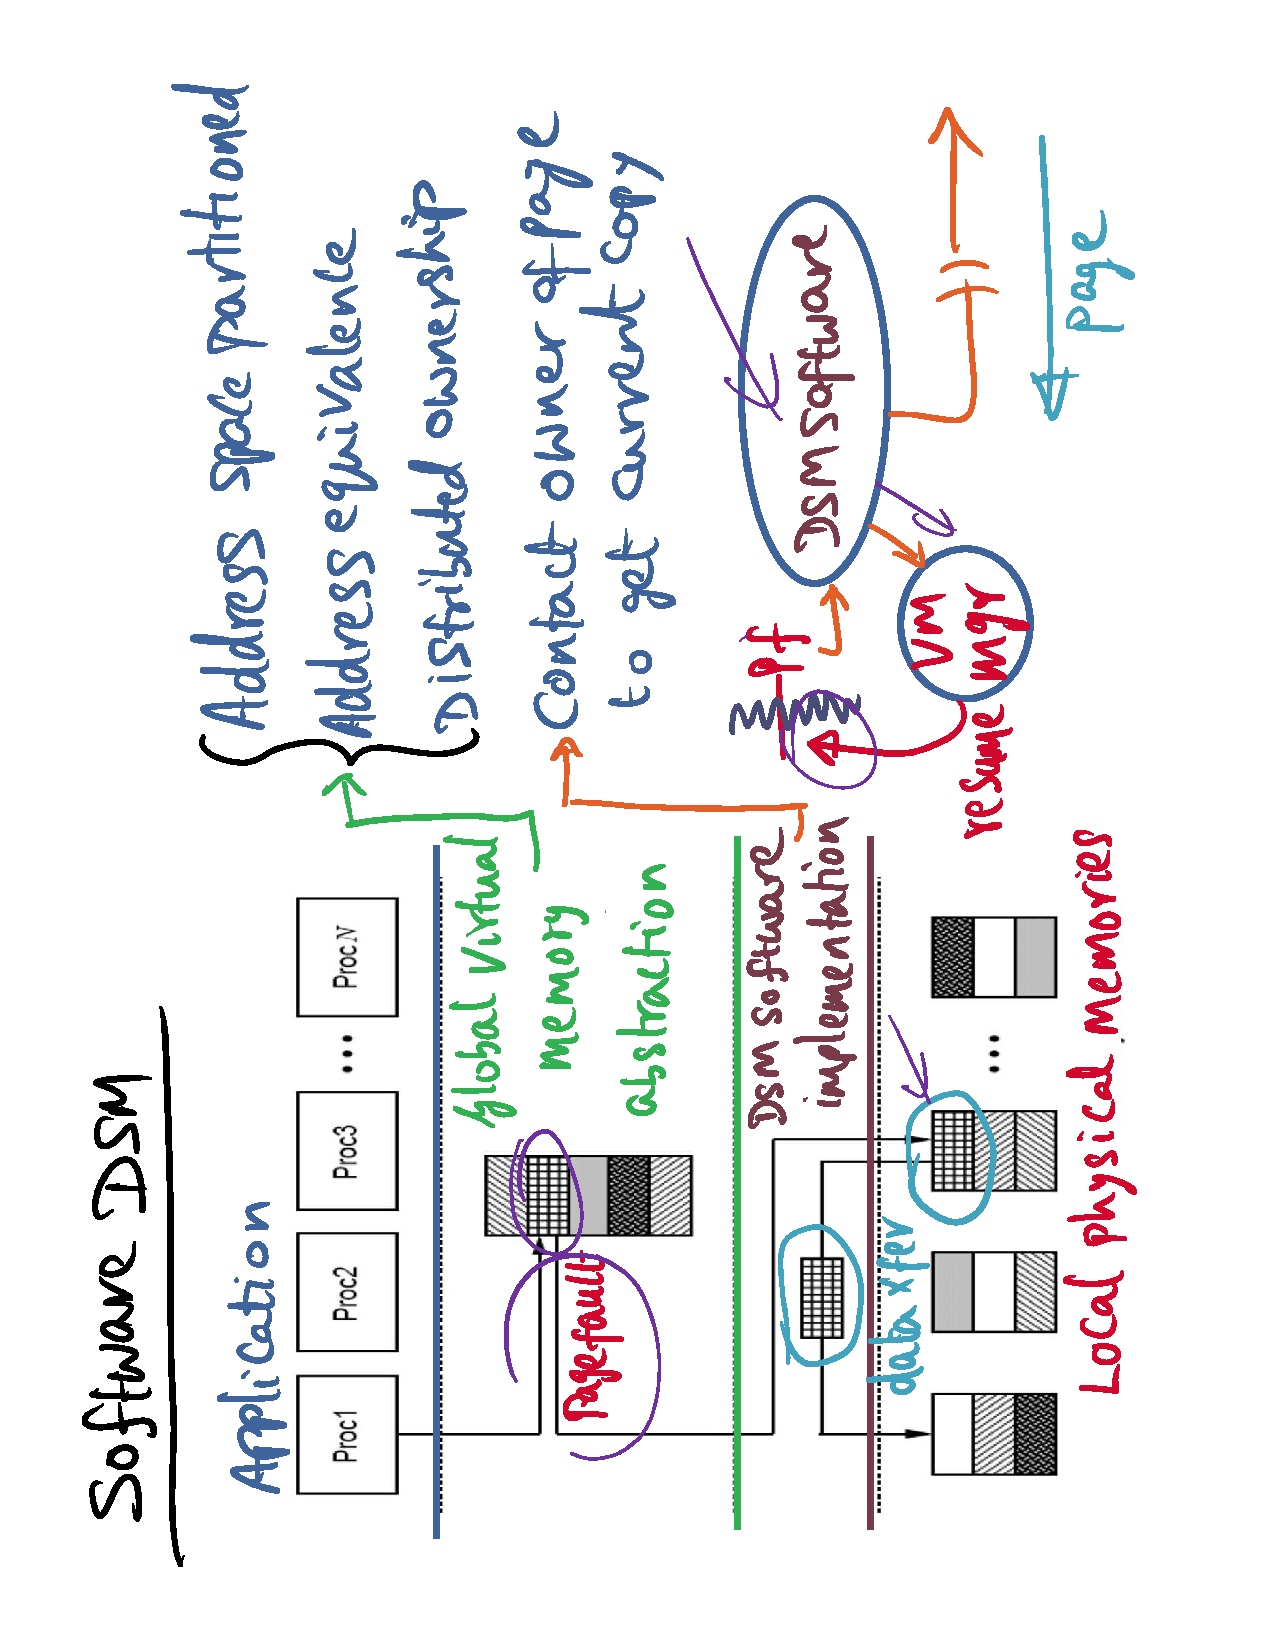
\includegraphics[width=\fullsize,angle=-90]{Figures/SoftDSM}
\caption{Software DSM.}\label{fig: SDSM}
\end{figure}

\noindent
{\bf Single-Writer Protocol for Software DSM.} Now it is the time to dive into the software DSM shown in~\autoref{fig: SDSM}. 
As you can see there are several layers in the software DSM. The one between the blue line and the green line 
is the abstraction layer seen by the application, which is giving this illusion of a global virtual memory. The 
next layer ({\it i.e.,} the next one below the abstraction layer) is the DSM software implementation layer, 
which implements this global virtual memory abstraction. In particular, this DSM software layer, which 
exists on every processor, knows that the point of access to a page by a processor, who exactly to contact, as 
the owner of the page, to get the current copy of the page. For instance, suppose there was a page fault 
on processor $1$. For a particular portion of the global address space. That portion of the global address space 
is currently not resident in $P1$'s local physical memory. So there is a page fault, and there is cooperation, as 
mentioned earlier, between the operating system and the DSM software. So when the page fault happens, the page fault is 
going to be communicated by the operating system to the DSM software. What the DSM software is going to do is, it knows 
the owner f the page, and so it is going to contact the owner of the page. And ask the owner to get the current 
copy of the page. Note that, the owner itself might not have the current copy of the page, but it knows which 
node has, and if that is the case, the owner is going to fetch the current copy of the page and 
send over to the node that is requesting it. Once the page is brought in the physical memory, the DSM 
software contacts the virtual memory manager notifying that it has completed and asking the virtual 
memory manager to update the page table of that processor so that it can resume execution. Then, 
the VM manager gets into action and updates the page table for the thread to indicate that the faulty virtual page is 
now mapped to a physical page. And then the processor or the thread can resume its execution. So that is the way 
coherence is going to be maintained by the DSM software and the cooperation between DSM software and the VM 
manager. And the coherence maintenance is happening at the level of individual pages. 

Early examples of 
systems that built software DSM include IVY from Yale~\cite{ivy}, CLOUDS from Georgia Tech.~\cite{clouds}, 
Mirage from UPenn~\cite{mirage}, and Munin from Rice~\cite{munin}. All of these are distributed shared systems and they 
all used coherence maintenance at the granularity of an individual page, and they used a protocol which 
is often referred to as a single-writer protocol. That is, as mentioned that the directory associated with 
the portion of the virtual memory space managed by each one of the nodes. And the directory has information 
as to who all are sharing a page at any point of time. Multiple readers can share a page at any point of time, 
but a single writer is only allowed to have the page at any point of time. So if there is a writer for a particular page, 
say that page is now currently in the memory of two different processors, if the writer wants to write 
to this page, then it has to inform through the DSM software abstraction, inform the owner of this page. Then, 
the owner is going to invalidate all copies of this page that exists in the entire system. So that 
this writer has exclusive access to that page so that it can make modifications to it. That is the single writer 
multiple reader protocol. 

Unfortunately, there is a ``problem'' with the single writer protocol. That is there is potential for 
what is called false sharing, which we have talked about already in the context of shared memory multiprocessor 
systems. Basically the concept of false sharing is that data appears to be shared even though programmatically they 
are not. Considering this page-based coherence maintenance. In the page-based coherence, 
the coherence maintenance that is done by the software, {\it i.e.,} DSM software, is of the granularity 
of a single page. A page may be $4K$ or $8K$ bytes, depending on the architecture. Clearly, within a page, 
lots of different data structures can actually fit. So if the coherence maintenance is being done at 
the level of an individual page, then we are invalidating copies of the page in several nodes to allow one 
writer to make modifications to some portions of the page. And that can be very severe in a page based 
system due the coarse granularity of the coherence information. So for example, this one page may 
contain ten different data structures, each of which is governed by a distinct lock as far as 
the application programmer is concerned. But even if I get a lock, which is for a particular data 
structure that happens to be in this page. And some other processor has a lock for a different data structure which is 
also on this page. When I get the lock that is going to manipulate a particular data structure in this 
page, and if I want to make modifications to it, I am going to go and invalidate all the other copies. 
When the other processor wants to make a change, it is going to come and invalidate my copy 
of this page. So the page can be ping-pong between multiple processors. Even though they are modifying 
different portions of the same page. Still the coherence granularity being a page, will results in this 
page shuttling back and forth between these two processors, even though the application program 
is perfectly well behaved in terms of using locks to govern different data structures. Unfortunately, all 
of the data structures happened to fit within the same page, resulting in this false sharing. Therefore, 
page-level granularity and single writer multiple reader protocol do not live happily together. 
They will lead to false sharing and ping-pong of the pages due to the false sharing among the 
threads of the application across the entire network.

In the next lecture, we will cover a solution to mitigate the false sharing issue of the single 
writer multiple reader protocol, and some implementation details.



\bibliographystyle{IEEEtran}
\bibliography{references}

\end{document}
